\section{Multipartite structure and implementation}
\label{physics:section}

The preceding construction controls the common one-qubit geometry. We now determine the multipartite entanglement of the measurement states and then examine the phase factorization and Clifford hierarchy of the measurement unitary.

\subsection{Genuine multipartite entanglement}
\label{physics:entanglement}
\label{physics:endpoints}

We first show directly that every measurement column is genuinely multipartite entangled for every $n\ge5$ and every real $t$. Write $\psi(y)=\braket{y}{\psi_0(t)}$ and $u=e^{it}$. Undoing the CNOT chain in Eq.~\eqref{core:phase-family} gives $w_j=y_j\oplus y_{j+1}$ for $j<n$; set $w^{(b)}=(w_1,\ldots,w_{n-1},b)$. The Hadamard on the last qubit then gives
\[
 \sqrt{2^{n+1}}\,\psi(y)
 =D_{n,t}(w^{(0)})+(-1)^{y_n}D_{n,t}(w^{(1)}).
\]
For $y=1^n$, the two input strings are $0^n$ and $e_n$, both with phase $1$, so $\psi(1^n)=0$. For a single flip $y=1^n\oplus e_j$, substitution in the kernel~\eqref{core:kernel} gives $d_n=0$ on both inputs of weights $1,2$ when $j=1,n$, and $d_n=1$ on both inputs of weights $2,3$ when $2\le j\le n-1$. Their phases are therefore $1,i$ or $iu,-u$, respectively. The sums or differences have modulus $\sqrt2$, hence $|\psi(1^n\oplus e_j)|=2^{-n/2}$ for every $j$.

For any nontrivial cut $A|B$, arrange the amplitudes as a matrix $V_A$, with $A$ labeling its rows and $B$ its columns. Choose $j\in A$ and $k\in B$. The rows $1_A,1_A\oplus e_j$ and columns $1_B,1_B\oplus e_k$ give
\[
 \begin{aligned}
 &\det\begin{pmatrix}
 0&\psi(1^n\oplus e_k)\\
 \psi(1^n\oplus e_j)&\psi(1^n\oplus e_j\oplus e_k)
 \end{pmatrix}\\
 &\qquad=-\psi(1^n\oplus e_j)\psi(1^n\oplus e_k).
 \end{aligned}
\]
Its modulus is $2^{-n}>0$, so $V_A$ has rank at least two and the seed is entangled across every cut. The local Pauli orbit~\eqref{core:orbit} preserves the Schmidt spectra and transfers this conclusion to every column.

To quantify this entanglement, write $p_A=\Tr\rho_A^2$ for a nonempty proper subsystem $A$. The genuine multipartite concurrence is~\cite{Ma2011}
\begin{equation}
 C_{\rm GME}(\psi)=\min_{\varnothing\ne A\subsetneq[n]}
 \sqrt{2(1-p_A)}.
 \label{physics:gme}
\end{equation}
This minimum measures entanglement across the weakest bipartition. For every $n\ge5$, every real $t$, and every column $k$, its exact value is
\begin{equation}
 C_{\rm GME}(\psi_k(t))=\sqrt{1-r_n(t)^2}>0.
 \label{physics:gme-law}
\end{equation}
Determining this value requires comparing all cut purities. Appendix~\ref{physics:app-purity} proves that every cut with at least two qubits on each side has purity strictly below $1/2$, whereas every one-qubit reduction has purity $(1+r_n(t)^2)/2\ge1/2$. The minimizing cuts are therefore precisely the $1|(n-1)$ cuts. Within this family, the common local radius thus determines the genuine multipartite concurrence. In particular, the enhanced endpoint, whose radius equals $r_E(n-1)$, is genuinely multipartite entangled and therefore not a product extension of a smaller EJM.

At $t=\pi/2$, every column has $C_{\rm GME}=1$ and is $1$-uniform~\cite{Scott2004}: all one-qubit reductions are $I/2$. Equation~\eqref{physics:endpoint-pair-purity} gives $p_{12}=11/32$ for $n=5$ and $p_{12}=5/16$ for every $n\ge6$. Both exceed $1/4$, so the endpoint is not $2$-uniform. Moreover, every two-qubit reduction of a stabilizer pure state has integer $4p_{ij}$, whereas these values give $11/8$ and $5/4$. Local unitaries preserve reduced purities and permutations only relabel the pairs. Thus, for every $n\ge5$, even allowing qubit permutations, no column at this endpoint is locally unitarily equivalent to a stabilizer pure state; see Appendix~\ref{physics:app-invariants} for the proof.

The zero-radius endpoints also distinguish the unified family from the even-qubit cosine family~\cite{PauwelsGisin2026}. For the cosine endpoint $\alpha=\pi/2$ at even $n\ge4$, $p_{12}=1/2+2^{3-n}$ and hence $C_{\rm GME}\le\sqrt{1-2^{4-n}}<1$, recovering the two-Bell-pair factorization at $n=4$. Thus, for every even $n\ge6$, the two endpoints have identical one-qubit reductions but are inequivalent under local unitaries and qubit permutations; see Appendix~\ref{physics:app-invariants}.

\subsection{Phase factorization and Clifford hierarchy}
\label{physics:implementation}

The complete phase separates into the four-feature kernel and a correction at the physical zero string. Substituting $f_0(z)=|z|-1+\delta_{z,0}\pmod4$ and $d_n(z)=q_n(z)-\delta_{z,0}$ into $D_{n,t}(z)=i^{f_0(z)}e^{itd_n(z)}$ gives
\begin{equation}
 D_{n,t}=-iP^{\otimes n}e^{itq_n}e^{i(\pi/2-t)Z_0},
 \label{physics:factorization}
\end{equation}
where $P=\operatorname{diag}(1,i)$, $Z_0=\ket{0^n}\bra{0^n}$, and $q_n$ denotes the diagonal operator of the Boolean kernel. Figure~\ref{fig:clifford}(a) gives the five-qubit seed preparation sequence, while panel (b) separates the complete diagonal phase for any $n\ge5$ into local $P$ gates, the four-feature kernel phase, and the zero-string conditional phase. The kernel phase is implemented by computing four parity checks into four clean auxiliaries, applying $e^{itF}$, and uncomputing the checks; computation and uncomputation use $O(n)$ CNOTs and restore the auxiliaries to zero. The additional gate $R_0(\theta)=e^{i\theta Z_0}$ is an $n$-qubit controlled phase, implementable with one clean ancilla and $O(n)$ elementary gates~\cite{Barenco1995}. The zero-string conditional phase has angle $\pi/2-t$: at the reference point $t=0$ and the enhanced endpoint $t=-\pi/2$, it gives the complete measurement unitary exact Clifford-hierarchy levels $n+1$ and $n$, respectively. At the zero-radius endpoint $t=\pi/2$, this conditional phase disappears and the level drops to four, independently of $n$.

For a diagonal gate $i^{f(z)}$, the Clifford-hierarchy criterion assigns a nonconstant mod-four monomial on $S$ weighted degree $|S|+1$ for an odd coefficient and $|S|$ for coefficient $2$; the largest weighted degree gives the exact level~\cite{GottesmanChuang1999,Cui2017}. At $t=0$, $\delta_{z,0}=\prod_j(1-z_j)$ contributes a degree-$n$ monomial with odd coefficient, giving level $n+1$. At $t=-\pi/2$, its coefficient is doubled, giving level $n$. At $t=\pi/2$, the zero-string correction vanishes. The mod-four polynomial of $F$ has degree three with an odd cubic coefficient, so its exact level is four. The four independent parity coordinates extend to an invertible binary change of variables, implemented by Clifford gates, which preserves this level when $F$ is pulled back to $q_n$. For $n\ge5$, the level-four kernel cannot cancel the higher-level zero-string term at the enhanced endpoint. The local factor $P^{\otimes n}$ and the Clifford factors $C_n,H^{\otimes n}$ also preserve these levels. Consequently the complete measurement unitary satisfies
\begin{equation}
 \begin{aligned}
 \ell(M_n(0))&=n+1,\\
 \ell(M_n(-\pi/2))&=n,\\
 \ell(M_n(\pi/2))&=4.
 \end{aligned}
 \label{physics:levels}
\end{equation}
\par
\onecolumngrid
\medskip
\noindent\begin{minipage}{\textwidth}
  \centering
  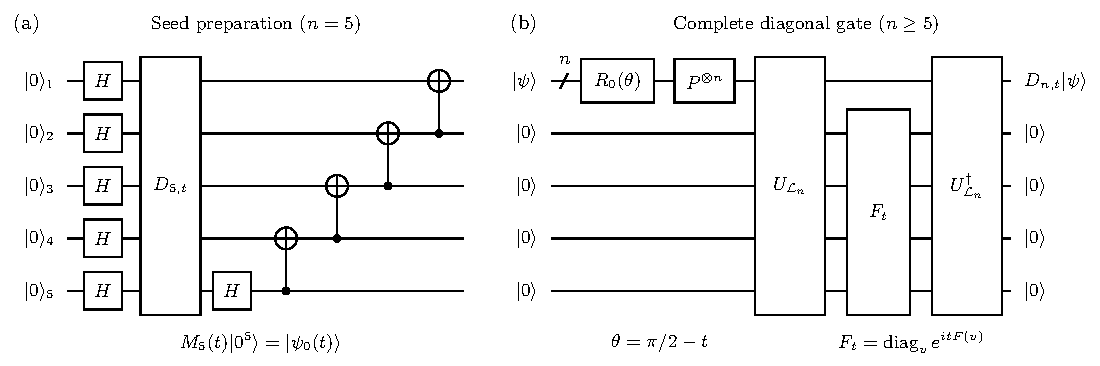
\includegraphics[width=\textwidth]{figures/fig4_clifford.pdf}
  \captionof{figure}{Circuit structure of the measurement unitary. Gates act from left to right.
  (a) Five-qubit seed preparation in the normal form of Ref.~\cite{PauwelsGisin2026}.
  (b) Decomposition of $D_{n,t}$ for every $n\ge5$, with the global phase $-i$ omitted.
  The top wire carries the $n$ data qubits, $P=\operatorname{diag}(1,i)$, and $R_0(\theta)=\exp(i\theta|0^n\rangle\langle0^n|)$ with $\theta=\pi/2-t$.
  $R_0$ is shown as an undecomposed $n$-qubit gate. Its implementation uses one clean ancilla; any of the four auxiliaries, still in $|0\rangle$ at that stage, can serve this role.
  The parity encoding $U_{\mathcal L_n}:|z\rangle|a\rangle\mapsto|z\rangle|a\oplus\mathcal L_nz\rangle$, the four-qubit gate $F_t$, and the inverse encoding implement $e^{itq_n}$ and restore the auxiliaries to $|0\rangle$.
  At $t=0$, $F_t=I$ and the encoding cancels with its inverse; $R_0(\pi/2)$ is the $X$-conjugated multi-controlled $P$ gate, recovering the decomposition of Ref.~\cite{PauwelsGisin2026}.
  At $t=\pi/2$, $R_0=I$.}
  \label{fig:clifford}
\end{minipage}
\par\medskip
\twocolumngrid


Appendix~\ref{physics:app-hierarchy} gives the full mod-four polynomial and derivation. In the localization framework of Refs.~\cite{PauwelsLocalization2025,PauwelsGisin2026}, these levels give upper bounds on the required resources.
